\documentclass[10pt]{article}
\usepackage[utf8]{inputenc}
\usepackage[T1]{fontenc}
\usepackage{amsmath}
\usepackage{amsfonts}
\usepackage{amssymb}
\usepackage[version=4]{mhchem}
\usepackage{stmaryrd}
\usepackage{hyperref}
\hypersetup{colorlinks=true, linkcolor=blue, filecolor=magenta, urlcolor=cyan,}
\urlstyle{same}
\usepackage{graphicx}
\usepackage[export]{adjustbox}
\graphicspath{ {./images/} }

\title{Distributed Robust Formation Flying and Attitude Synchronization of Spacecraft }


\author{Md Nur-A-Adam Dony ${ }^{1}$ and Wenjie Dong ${ }^{2}$}
\date{}


%New command to display footnote whose markers will always be hidden
\let\svthefootnote\thefootnote
\newcommand\blfootnotetext[1]{%
  \let\thefootnote\relax\footnote{#1}%
  \addtocounter{footnote}{-1}%
  \let\thefootnote\svthefootnote%
}

%Overriding the \footnotetext command to hide the marker if its value is `0`
\let\svfootnotetext\footnotetext
\renewcommand\footnotetext[2][?]{%
  \if\relax#1\relax%
    \ifnum\value{footnote}=0\blfootnotetext{#2}\else\svfootnotetext{#2}\fi%
  \else%
    \if?#1\ifnum\value{footnote}=0\blfootnotetext{#2}\else\svfootnotetext{#2}\fi%
    \else\svfootnotetext[#1]{#2}\fi%
  \fi
}

\begin{document}
\maketitle


\begin{abstract}
This paper considers the spacecraft formation flying (SFF) with a desired attitude. Two control problems are studied. One is the formation control of multiple spacecraft and the other is the attitude synchronization of multiple spacecraft. To solve the two problems, a 6-DOF model is adopted for each spacecraft. In the 6-DOF model, it is assumed that the inertia parameters are not well known and there are perturbations of orbitals, gravity, etc. With the aid of the backstepping technique and the algebraic graph theory, distributed robust control laws are proposed for the formation flying and attitude synchronization problems, respectively. The effectiveness of the proposed controllers is shown by simulation. DOI: 10.1061/(ASCE)AS.1943-5525.0001262. ㅇ 2021 American Society of Civil Engineers.
\end{abstract}

Author keywords: Spacecraft; Formation flying; Attitude synchronization; Distributed control; Cooperative control; Robust control.

\section{Introduction}
The spacecraft formation flying (SFF) is a technology that makes smaller and inexpensive spacecraft work cooperatively to accomplish complex tasks. SFF has some advantages such as the robustness toward failure of individual systems, increased flexibility, scalability in deployment of systems, etc. SFF is useful in many activities. For example, it can be used in remote sensing of the Earth, interferometric measurements, gravitational waves measurements, building of the space stations in orbit, etc. For SFF, it is important to control the relative positions and attitudes of all spacecraft. However, precise control of positions and attitude of multiple spacecraft is challenging due to the nonlinear feature of the dynamics of each spacecraft, perturbations of spacecraft orbits, and limited communication between spacecraft.

SFF was studied in Clohessy and Wiltshire (1960) by considering each spacecraft as a linear system. Considering the nonlinear nature of the model of a spacecraft and uncertainty in the model, SFF has been studied with the aid of nonlinear models of the relative translation in Haizhou and Kapila (2001), Wang and Hadaegh (1996), and Yan et al. (2000b). Several nonlinear controllers have been proposed with the aid of the nonlinear control theory. Simultaneous control of relative positions and attitudes of spacecraft has also been studied and is called 6-DOF SFF in Kristiansen et al. (2008), Wang and Sun (2012), Sun et al. (2011), Lv et al. (2011), and Lan et al. (2015). In Kristiansen et al. (2008), several nonlinear controllers were proposed. In Lv et al. (2011), input constraints and uncertainties were considered and nonlinear controllers were proposed. In Wang and Sun (2012) and Lan et al. (2015), finite-time tracking controllers were proposed. In the aforementioned literature, it is always assumed that there are one leader spacecraft

\footnotetext{${ }^{1}$ Graduate Student, Dept. of Electrical and Computer Engineering, Univ. of Texas Rio Grande Valley, Edinburg, TX 79539. Email: mdnuraadam \href{mailto:.dony01@utrgv.edu}{.dony01@utrgv.edu}

${ }^{2}$ Professor, Dept. of Electrical and Computer Engineering, Univ. of Texas Rio Grande Valley, Edinburg, TX 79539 (corresponding author). Email: \href{mailto:wenjie.dong@utrgv.edu}{wenjie.dong@utrgv.edu}

Note. This manuscript was submitted on February 25, 2020; approved on November 25, 2020; published online on February 25, 2021. Discussion period open until July 25, 2021; separate discussions must be submitted for individual papers. This paper is part of the Journal of Aerospace Engineering, (C) ASCE, ISSN 0893-1321.
}and one follower spacecraft, and a controller is designed such that the follower spacecraft follows the leader spacecraft. In some practical applications the number of the follower spacecraft is larger than one. However, the SFF problem has not been well solved for multiple follower spacecraft.

Recently cooperative control of multiple agents (or systems) has been an active area of research. Several control methods have been developed. Desai et al. (1998, 2001), Mesbahi and Hadaegh (2001), and Wang and Hadaegh (1996) developed the leader-following approach; Balch and Arkin (1998), Jonathan et al. (2003), Lawton et al. (2003), and Sugihara and Suzuki (1996) developed the behavioral approach; Beard et al. (2001), Lewis and Tan (1997), and Ren and Beard (2004) developed the virtual structure approach; and Das et al. (2002), Eren et al. (2002), Fax and Murray (2004), Lafferriere et al. $(2004,2005)$, and Olfati-Saber and Murray (2002) developed the graph approach. The graph approach has been applied to solve the consensus problems of multiagent systems with or without a leader. Olfati-Saber and Murray (2002), Ren and Beard (2005), Li et al. (2010), Scardovi and Sepulchre (2009), and Wieland et al. (2011) solved the consensus problem of multiple linear systems based on different assumptions. For the consensus of multiple nonlinear systems, distributed control laws were proposed in Lee and Ahn (2010), Qu (2010), and Zhang and Lewis (2012). The consensus problem of multiple systems with a leader has been studied in Hong et al. (2006, 2008), Cao and Ren (2010a, b), Mei et al. (2011), and Dong (2013), and distributed controllers were proposed based on different assumptions.

In this paper, we consider SFF with multiple followers. The communication between spacecraft is defined by a directed graph. The SFF problems are considered as a formation control problem and an attitude consensus problem of multiple spacecraft with a leader spacecraft. The dynamics for each spacecraft are assumed to be a 6-DOF model with parametric and nonparametric uncertainties. For the formation control problem, distributed robust adaptive control laws are proposed so that the spacecraft come into a desired formation whose motion is defined by the leader spacecraft. For the attitude consensus problem, distributed robust controllers are proposed with the aid of quaternion so that the attitudes of all spacecraft converge to the attitude of the leader spacecraft. Simulation has been done to verify the effectiveness of the proposed control laws. The contributions of this paper are as follows: - For each follower spacecraft, a distributed position control law and a distributed attitude control law are proposed for formation flying with a desired attitude with the aid of the backstepping technique and distributed estimation. The proposed control laws work well for any finite number of follower spacecraft. While in Haizhou and Kapila (2001), Wang and Hadaegh (1996), Yan et al. (2000a), Kristiansen et al. (2008), Wang and Sun (2012), Sun et al. (2011), Lv et al. (2011), and Lan et al. (2015) the formation flying is considered for one follower spacecraft. Moreover, the proposed control laws in this paper are for directed communication graphs. No bidirectional communication between spacecraft is required.

\begin{itemize}
  \item The proposed control laws are robust to both inertia parameters and disturbance. Exact knowledge of the inertia parameters and disturbance is not required. In Ren and Beard (2004) and Wang and Hadaegh (1996), the research on the formation control is based on the exact knowledge of the system model. In Mercier et al. (2020), robust distributed control laws were proposed for the problem considered in this paper. However, the magnitudes of the distributed control laws for the relative translation are larger than those in this paper. This is because in this paper neural networks are introduced to learn the uncertain terms while in Mercier et al. (2020) the unknown terms are dominated by a sign function with large magnitude. The distributed control laws for the attitude synchronization in this paper are globally defined because they are proposed based on quaternion. While the distributed control laws for the attitude synchronization in Mercier et al. (2020) are not well defined for all configurations (i.e., singular for some configurations) because they were proposed based on Euler angles.
\end{itemize}

The rest of this paper is organized as follows. In Section 2, "Problem Statement," the dynamics of spacecraft and the problem considered in this paper are presented. In Section 3, "Distributed Controller Design for Relative Translation," distributed controllers are proposed for formation control. In Section 4, "Distributed Controller Design for Attitude Control" distributed controllers are proposed for attitude control. In Section 5, "Simulation," simulation results are given. The last section concludes this paper.

\section{Problem Statement}
\section{Relative Translation Dynamics}
Define an earth-centered inertial $(\mathrm{ECI})$ frame $\mathcal{F}_{I}$ with the origin in the center of the Earth, $z$-axis being the rotation axis of the Earth toward the celestial north pole, $x$-axis directing toward the vernal equinox, and $y$-axis determined by the $x$ - and $z$ - axes using the right hand.

Let $\mathbf{r}$ be the position of the mass center of the chief spacecraft in the ECI frame. Define a reference frame $\mathcal{F}_{c}$ with the origin in the mass center of the chief spacecraft, $x$-axis defined by vector $\mathbf{r} /\|\mathbf{r}\|$, $z$-axis defined by vector $(\mathbf{r} \times \dot{\mathbf{r}}) /(\|\mathbf{r} \times \dot{\mathbf{r}}\|)$, and the $y$-axis determined by the $x$ - and $z$ - axes using the right hand. For the convenience of presentation, it is assumed that the chief spacecraft moves in frame $\mathcal{F}_{c}$ and the control input of the chief spacecraft is zero.

Assume there are $m$ small spacecraft that move around the chief spacecraft. The dynamics of the relative translation of $j$-th spacecraft are [see Yan et al. (2000a) and Kapilal et al. (1999)]

$$
m_{j} \ddot{p}_{j}+C_{j}(\dot{\nu}) \dot{p}_{j}+D_{j}\left(\dot{\nu}, \ddot{\nu}, r_{r}, p_{j}\right)=F_{j}+F_{d j}
$$

where $p_{j} \in R^{3}=$ relative position of the $j$-th spacecraft in frame $\mathcal{F}_{c} ; m_{j}=$ mass of the $j$-th spacecraft; and $r_{r}$ and $r_{j}=$ distance of the chief spacecraft and $j$-th spacecraft to the center of the earth, respectively.

$$
\begin{gathered}
\ddot{r}_{r}=r_{r} \dot{\nu}^{2}-\mu \frac{1}{r_{r}^{2}} \\
\ddot{\nu}=-\frac{2 \dot{r}_{r} \dot{\nu}}{r_{r}}
\end{gathered}
$$

where $\nu=$ true anomaly of the chief spacecraft; $\mu=M g, M$ is the Earth's mass; and $g=$ universal gravity constant, $r_{r}=\|\mathbf{r}\|$

$$
C_{j}(\dot{\nu})=2 m_{j} \dot{\nu}\left[\begin{array}{ccc}
0 & -1 & 0 \\
1 & 0 & 0 \\
0 & 0 & 0
\end{array}\right]
$$

is a Coriolis-like matrix

$$
D_{j}\left(\dot{\nu}, \ddot{\nu}, r_{r}, p_{j}\right)=m_{j}\left[\begin{array}{c}
\frac{\mu\left(p_{1 j}+r_{r}\right)}{\left[\left(r_{r}+p_{1 j}\right)^{2}+p_{2 j}^{2}+p_{3 j}^{2}\right]^{\frac{3}{2}}}-\frac{\mu}{r_{r}^{2}}-\dot{\nu}^{2} p_{1 j}+\ddot{\nu} p_{2 j} \\
\frac{\mu p_{2 j}}{\left[\left(r_{r}+p_{1 j}\right)^{2}+p_{2 j}^{2}+p_{3 j}^{2}\right]^{\frac{3}{2}}}-\dot{\nu}^{2} p_{2 j}-\ddot{\nu} p_{1 j} \\
\frac{\mu p_{3 j}}{\left[\left(r_{r}+p_{1 j}\right)^{2}+p_{2 j}^{2}+p_{3 j}^{2}\right]^{\frac{3}{2}}}
\end{array}\right]
$$

where $F_{d j}=$ disturbance; and $F_{j}=$ control input.

For the dynamics (1), the following two properties are useful.

Property 1: $C_{j}=$ skew-symmetric matrix.

Property 2: For any two vectors, $x=\left[x_{1}, x_{2}, x_{3}\right]^{\mathrm{T}} \in R^{3}$; and $y=\left[y_{1}, y_{2}, y_{3}\right]^{\mathrm{T}} \in R^{3}$

$$
m_{j} x+C_{j}(\dot{\nu}) y+D_{j}\left(\dot{\nu}, \ddot{\nu}, r_{r}, p_{j}\right)=Y_{1 j}\left(p_{j}, x, y\right) m_{j}
$$

where

$$
\begin{aligned}
& Y_{1 j}\left(p_{j}, x, y\right) \\
& =\left[\begin{array}{c}
x_{1}-2 \dot{\nu} y_{2}+\frac{\mu\left(p_{1 j}+r_{r}\right)}{\left[\left(r_{r}+p_{1 j}\right)^{2}+p_{2 j}^{2}+p_{3 j}^{2}\right]^{\frac{3}{2}}}-\frac{\mu}{r_{r}^{2}}-\dot{\nu}^{2} p_{1 j}+\ddot{\nu} p_{2 j} \\
x_{2}+\dot{\nu} y_{1}+\frac{\mu p_{2 j}}{\left[\left(r_{r}+p_{1 j}\right)^{2}+p_{2 j}^{2}+p_{3 j}^{2}\right]^{\frac{3}{2}}}-\dot{\nu}^{2} p_{2 j}-\ddot{\nu} p_{1 j} \\
x_{3}+\frac{\mu p_{3 j}}{\left[\left(r_{r}+p_{1 j}\right)^{2}+p_{2 j}^{2}+p_{3 j}^{2}\right]^{\frac{3}{2}}}
\end{array}\right]
\end{aligned}
$$

is the regressor matrix.

\section{Dynamics of Attitude}
For spacecraft $j$, define a body frame $\mathcal{F}_{b j}$ with the origin in the mass center of the spacecraft; the $x-, y$-, and $z$ - axes are attached to the spacecraft body and coincide with the principal axis of inertia of the spacecraft. The rotation matrix of frame $\mathcal{F}_{b j}$ with respect to frame $\mathcal{F}_{I}$ is denoted by $R_{j}$. The angular velocity of the spacecraft $j$ with respect to the ECI frame $\mathcal{F}_{I}$ is denoted by $\omega_{j}=$ $\left[\omega_{1 j}, \omega_{2 j}, \omega_{3 j}\right]^{T}$. The kinematics of spacecraft $j$ is

$$
\dot{R}_{j}=R_{j} S\left(\omega_{j}\right)
$$

where $S\left(\omega_{j}\right)=$ skew-symmetric matrix defined as

$$
S\left(\omega_{j}\right)=\left[\begin{array}{ccc}
0 & -\omega_{3 j} & \omega_{2 j} \\
\omega_{3 j} & 0 & -\omega_{1 j} \\
-\omega_{2 j} & \omega_{1 j} & 0
\end{array}\right]
$$

The dynamics of the attitude is

$$
J_{j} \dot{\omega}_{j}=-S\left(\omega_{j}\right) J_{j} \omega_{j}+\tau_{j}+\tau_{d j}
$$

where $J_{j}=$ moment of inertia; $\tau_{j}=$ torque input; and $\tau_{d j}=$ disturbance.

The attitude of $j$-th spacecraft can also be represented by a unit quaternion $q_{j}=\left[\eta_{j}, \epsilon_{j}^{\mathrm{T}}\right]^{\mathrm{T}} \in R^{4}$. The relation between $R_{j}$ and $q_{j}$ is

$$
R_{j}=I_{3}+2 \eta_{j} S\left(\epsilon_{j}\right)+2 S\left(\epsilon_{j}\right)^{2}
$$

Eq. (8) is equivalent to

$$
\dot{q}_{j}=\frac{1}{2} A\left(q_{j}\right) \omega_{j}
$$

where

$$
A\left(q_{j}\right)=\left[\begin{array}{c}
-\epsilon_{j}^{\mathrm{T}} \\
\eta_{j} I_{3}+S\left(\epsilon_{j}\right)
\end{array}\right]
$$

Let the relative attitude be

$$
\tilde{q}_{j}=\left[\tilde{\eta}_{j}, \tilde{\epsilon}_{j}^{\mathrm{T}}\right]^{\mathrm{T}}=q_{r}^{-1} \otimes q_{j}
$$

where $q_{r}=$ unit quaternion of the chief spacecraft with respect to ECI, then

$$
\dot{\tilde{q}}_{j}=\frac{1}{2} A\left(\tilde{q}_{j}\right) \tilde{\omega}_{j}
$$

where

$$
\tilde{\omega}_{j}=\omega_{j}-\tilde{R}_{j}^{\mathrm{T}} \omega_{r}
$$

In which $\tilde{R}_{j}=$ rotation matrix corresponding to the quaternion $\tilde{q}_{j}$; and $\omega_{r}=$ angular velocity of the chief spacecraft with respect to ECI. Then

$$
J_{j} \dot{\tilde{\omega}}_{j}+N_{j}\left(\tilde{R}_{j}, \tilde{\omega}_{j}, \omega_{r}\right) \tilde{\omega}_{j}+G_{j}\left(\tilde{R}_{j}, \omega_{r}, \dot{\omega}_{r}\right)=\tau_{j}+\tau_{d j}
$$

where

$$
\begin{aligned}
& N_{j}\left(\tilde{R}_{j}, \tilde{\omega}_{j}, \omega_{r}\right)=-S\left(J_{j} \tilde{\omega}_{j}\right)-S\left(J_{j} \tilde{R}_{j}^{\mathrm{T}} \omega_{r}\right)+S\left(\tilde{R}_{j}^{\mathrm{T}} \omega_{r}\right) J_{j} \\
&+J_{j} S\left(\tilde{R}_{j}^{\mathrm{T}} \omega_{r}\right) \\
& G_{j}\left(\tilde{R}_{j}, \omega_{r}, \dot{\omega}_{r}\right)=S\left(\tilde{R}_{j}^{\mathrm{T}} \omega_{r}\right) J_{j} \tilde{R}_{j}^{\mathrm{T}} \omega_{r}+J_{j} \tilde{R}_{j}^{\mathrm{T}} \dot{\omega}_{r}
\end{aligned}
$$

For the dynamics in Eq. (17), the following two properties are useful.

Property 3: $N_{j}$ is a skew-symmetric matrix.

Property 4: For any two vectors, $x=\left[x_{1}, x_{2}, x_{3}\right]^{\mathrm{T}} \in R^{3}$; and $y=\left[y_{1}, y_{2}, y_{3}\right]^{\mathrm{T}} \in R^{3}$

$J_{j} x+N_{j}\left(\tilde{R}_{j}, \tilde{\omega}_{j}, \omega_{r}\right) y+G_{j}\left(\tilde{R}_{j}, \omega_{r}, \dot{\omega}_{r}\right)=Y_{2 j}\left(\tilde{R}_{j}, \tilde{\omega}_{j}, x, y\right) a_{j}$

where $a_{j}=\operatorname{vec}\left(J_{j}\right)$

$$
\begin{aligned}
Y_{2 j}\left(\tilde{R}_{j}, \tilde{\omega}_{j}, x, y\right)= & \Gamma(x)+S(y) \Gamma\left(\tilde{\omega}_{j}\right)+S(y) \Gamma\left(\tilde{R}_{j}^{\mathrm{T}} \omega_{r}\right) \\
& +S\left(\tilde{R}_{j}^{\mathrm{T}} \omega_{r}\right) \Gamma(y)+\Gamma\left(S\left(\tilde{R}_{j}^{\mathrm{T}} \omega_{r}\right) y\right) \\
+ & S\left(\tilde{R}_{j}^{\mathrm{T}} \omega_{r}\right) \Gamma\left(\tilde{R}_{j}^{\mathrm{T}} \omega_{r}\right)+\Gamma\left(\tilde{R}_{j}^{\mathrm{T}} \dot{\omega}_{r}\right)
\end{aligned}
$$

is the regressor matrix and $\Gamma(x)=\operatorname{diag}(x)$.

\section{Communication between Spacecraft}
There are communications for multiple spacecraft. Label $m$ spacecraft by $1,2, \ldots, m$. The communication between the spacecraft can be defined by a directed graph (digraph) $\mathcal{G}=\{\mathcal{A}, \mathcal{E}\}$ where $\mathcal{A}=\{1,2, \ldots, m\}$ is the node set and $\mathcal{E}=\left\{e_{i j}\right\}_{1 \leq i, j \leq m}$ is the edge set. In digraph $\mathcal{G}$, the edge $e_{i j}$ is directed and means that the information of spacecraft $i$ is available to spacecraft $j$. If there is an edge $e_{i j}$, spacecraft $i$ is called a neighbor of spacecraft $j$. All neighbors of spacecraft $j$ form a set that is denoted by $\mathcal{N}_{j}$. A directed path from node $j$ to node $i$ is a sequence of edges that connect node $j$ and node $i$ with direction from node $j$ to node $i$. A node is said to be globally reachable if there exists a directed path from this node to all other nodes.

For a digraph $\mathcal{G}$, the weighted adjacent matrix $A=\left[a_{j i}\right] \in R^{n \times n}$ is defined by

$$
a_{j i}\left\{\begin{array}{l}
>0, \quad \text { if } e_{i j} \in \mathcal{E} \\
=0, \quad \text { if } e_{i j} \notin \mathcal{E} \quad \text { or } \quad i=j
\end{array}\right.
$$

The weighted Laplacian matrix of the digraph $\mathcal{G}$ with adjacent matrix $A$ is defined by

$$
L=A \mathbf{1}-A
$$

where $\mathbf{1}$ = vector with all elements being one.

Assume there is a leader spacecraft. The leader spacecraft is labeled 0 without loss of generalization, and the other spacecraft is called the follower spacecraft. The leader spacecraft does not have a neighbor, i.e., $\mathcal{N}_{0}=\emptyset$. The communication between $m$ follower spacecraft and the leader spacecraft can be described by an augmented digraph $\mathcal{G}^{e}=\left\{\mathcal{A}^{e}, \mathcal{E}^{e}\right\}$ where $\mathcal{A}^{e}=\mathcal{A} \cup\{0\}$ and $\mathcal{E}^{e}$ is the union of the elements in $\mathcal{E}$ and the edges that connect the leader spacecraft to the follower spacecraft. Fig. 1 is an example of the communication digraph for one leader spacecraft (node 0 ) and three follower spacecraft (nodes 1, 2, and 3). So, $\mathcal{A}^{e}=\{1,2,3,0\}$ and $\mathcal{E}^{e}=\left\{e_{21}, e_{23}, e_{32}, e_{03}, e_{01}\right\}$. This digraph shows that the information of the leader spacecraft is available to spacecraft 1 and 3 , the information of spacecraft 2 is available to spacecraft 1 and 3 , and the information of spacecraft 3 is available to spacecraft 2 . Therefore, $\mathcal{N}_{0}=\emptyset, \mathcal{N}_{1}=\{0\}, \mathcal{N}_{2}=\{3\}$, and $\mathcal{N}_{3}=\{0,2\}$. Also, node 0 is globally reachable because there is a directed path from node 0 to any other node.

A desired formation $\mathcal{F}$ of a leader spacecraft and $m$ follower spacecraft can be defined by a geometric pattern formed by the

\begin{center}
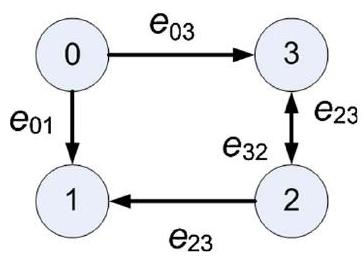
\includegraphics[max width=\textwidth]{2023_10_07_a50fd94fd281fe9896c1g-03}
\end{center}

Fig. 1. The communication digraph of one leader spacecraft and three follower spacecraft. points with the coordinates $h_{j}=\left[h_{x j}, h_{y j}, h_{z j}\right]^{\mathrm{T}} \in R^{3}$ for $0 \leq j \leq m$. The spacecraft are said in desired formation $\mathcal{F}$ if $p_{j}-p_{i}=h_{j}-h_{i}$ for all $0 \leq j, i \leq m$.

\section{Problem Definition}
In this paper, the following control problem is considered.

For $m$ spacecraft and one leader spacecraft with a communication digraph $\mathcal{G}^{e}$ and a desired formation $\mathcal{F}$, the distributed formation control problem with the desired attitude is to design a distributed control law for each follower spacecraft using its neighbors' information such that

$$
\begin{gathered}
\lim _{t \rightarrow \infty}\left(p_{j}-h_{j}-\left(p_{i}-h_{i}\right)\right)=0, \quad 0 \leq j, i \leq m \\
\lim _{t \rightarrow \infty} \tilde{q}_{i}^{-1} \tilde{q}_{j}=[1,0,0,0]^{\mathrm{T}}, \quad 1 \leq i, j \leq m
\end{gathered}
$$

In the preceding formation problem, Eq. (25) means that all spacecraft come into the desired formation $\mathcal{F}$. Eq. (26) means that the attitude of each follower spacecraft converges to the attitude of the leader spacecraft.

To solve the defined problem, we make the following assumptions:

Assumption 1 The inertia parameter $m_{j}$ is a constant and is unknown. Its nominal value is $\bar{m}_{j}$ and is known. Also, $\left|m_{j}-\bar{m}_{j}\right| \leq$ $\rho_{1 j}$ and $\rho_{1 j}$ is known.

Assumption 2 The inertia parameter $J_{j}$ is a diagonal constant matrix and is unknown. Its nominal value is $\bar{J}_{j}$ and is known. Also, $\left\|J_{j}-\bar{J}_{j}\right\| \leq \rho_{2 j}$ and $\rho_{2 j}$ is known.

Assumption 3 Disturbance $F_{d j}$ and $\tau_{d j}$ are bounded, i.e., $\left\|F_{d j}\right\| \leq \rho_{3 j}$ and $\left\|\tau_{d j}\right\| \leq \rho_{4 j}$, where $\rho_{3 j}$ and $\rho_{4 j}$ are known.

Assumption 4 The node 0 in the digraph $\mathcal{G}^{e}$ is globally reachable.

Assumption 5 For the leader spacecraft, $\left\|\ddot{p}_{0}-\ddot{h}_{0}\right\| \leq \rho_{5}$ and $\left\|\ddot{\tilde{q}}_{0}\right\| \leq \rho_{6}$, where $\rho_{5}$ and $\rho_{6}$ are known positive constants.

\section{Preliminary Results on Distributed Control}
For the digraph $\mathcal{G}^{e}$ with a weight matrix $A^{e}=\left[a_{j i}\right]_{(m+1) \times(m+1)}$ $\left(a_{j i}>0\right)$, its weighted Laplacian matrix $\mathcal{L}^{e}=\left[L_{j i}^{e}\right]_{(m+1) \times(m+1)}$ is defined as

$$
L_{j i}^{e}= \begin{cases}-a_{j i}, & \text { if } i \neq j \text { and } i \in \mathcal{N}_{j}^{e} \\ 0, & \text { if } i \neq j \text { and } i \notin \mathcal{N}_{j}^{e} \\ \sum_{k \in \mathcal{N}_{j}^{e}} a_{j k}, & \text { if } i=j\end{cases}
$$

For the digraph $\mathcal{G}$ with the weight matrix $A$, which is formed by the last $m$ rows and the last $m$ columns of $A^{e}$, its weighted Laplacian matrix $\mathcal{L}=\left[L_{j i}\right]_{m \times m}$ is defined as

$$
L_{j i}= \begin{cases}-a_{j i}, & \text { if } i \neq j \text { and } i \in \mathcal{N}_{j} \\ 0, & \text { if } i \notin j \text { and } i \notin \mathcal{N}_{j} \\ \sum_{k \in \mathcal{N}_{j}} a_{j k}, & \text { if } i=j\end{cases}
$$

By the definition

$$
\mathcal{L}^{e}=\left[\begin{array}{cc}
0 & \mathbf{0} \\
-\mathcal{L}_{21}^{e} & \mathcal{L}_{22}^{e}
\end{array}\right]=\left[\begin{array}{cc}
0 & \mathbf{0} \\
-\mathcal{L}_{21}^{e} & \mathcal{L}+\operatorname{diag}\left(\mathcal{L}_{21}^{e}\right)
\end{array}\right]
$$

where

$$
\begin{gathered}
\mathcal{L}_{22}^{e}=\mathcal{L}+\operatorname{diag}\left(\mathcal{L}_{21}^{e}\right) \\
\mathcal{L}_{21}^{e}=\left[a_{10}, \ldots, a_{m 0}\right]^{\mathrm{T}}
\end{gathered}
$$

and

$$
a_{j 0}\left\{\begin{array}{cc}
>0, & \text { if node } 0 \text { is available to node } j \\
=0, & \text { otherwise }
\end{array}\right.
$$

for $1 \leq j \leq m$.

For the weighted Laplacian matrix $\mathcal{L}^{e}$, the following results will be applied in this paper.

Lemma 1 [Qu (2009) and Dong (2013)] For the digraph $\mathcal{G}^{e}$ with weighted matrix $A^{e}=\left[a_{j i}\right]_{(m+1) \times(m+1)} \quad\left(a_{j i} \geq 0\right)$, its weighted Laplacian matrix $\mathcal{L}^{e}$ is defined in Eq. (27). If node 0 is globally reachable, then

\begin{enumerate}
  \item $-\mathcal{L}_{22}^{e}$ is a Hurwitz matrix; and

  \item Let

\end{enumerate}

$$
P=\left(\operatorname{diag}\left(\left(\mathcal{L}_{22}^{e}\right)^{-1} \mathbf{1}\right)\right)^{-1}=\operatorname{diag}\left(\left[P_{1}, \ldots, P_{m}\right]\right)
$$

then $P$ and

$$
Q=P \mathcal{L}_{22}^{e}+\left(\mathcal{L}_{22}^{e}\right)^{\mathrm{T}} P
$$

are positive definite matrices.

Lemma 2 [Dong (2013)] For $m$ follower systems with state $x_{j} \in \Re(1 \leq j \leq m)$ and a leader system with state $x_{0} \in \Re$, the communication between $(m+1)$ systems is described by a direct graph $\mathcal{G}^{e}$. It is assumed that the state of the leader system is globally reachable for each follower system.

\begin{enumerate}
  \item If $x_{0}$ is a constant; and
\end{enumerate}

$$
\dot{x}_{j}=-\sum_{i \in \mathcal{N}_{j}^{e}} a_{j i}\left(x_{j}-x_{i}\right), \quad 1 \leq j \leq m
$$

where constants $a_{j i}>0$, then $x_{j}-x_{0}$ exponentially converge to zero for $1 \leq j \leq m$.

\begin{enumerate}
  \setcounter{enumi}{1}
  \item If $x_{0}$ is time-varying, $\left|\dot{x}_{0}(t)\right| \leq \delta_{0}$ for all time, and
\end{enumerate}

$$
\begin{gathered}
\dot{x}_{j}=-\sum_{i \in \mathcal{N}_{j}^{e}} a_{j i}\left(x_{j}-x_{i}\right)-\delta_{j} \operatorname{sign}\left(\sum_{i \in \mathcal{N}_{j}^{e}} a_{j i}\left(x_{j}-x_{i}\right)\right) \\
\dot{\delta}_{j}=-\sum_{i \in \mathcal{N}_{j}^{e}} a_{j i}\left(\delta_{j}-\delta_{i}\right), \quad 1 \leq j \leq m
\end{gathered}
$$

where constants $a_{j i}>0$, then $x_{j}-x_{0}$ and $\delta_{j}-\delta_{0}$ exponentially converge to zero for $1 \leq j \leq m$.

\section{Distributed Controller Design for Relative Translation}
The distributed controller is designed in two steps. Step 1: Define

$$
\alpha_{j}=-\sum_{j \in \mathcal{N}_{j}} a_{j i}\left(p_{j}-h_{j}-\left(p_{i}-h_{i}\right)\right)+\dot{h}_{j}+\xi_{j}
$$

where $a_{j i}=$ positive constants; and $\xi_{j}=$ estimate of $\dot{p}_{0}-\dot{h}_{0}$ and will be designed in the next step. Let

$$
s_{j}=\dot{p}_{j}-\alpha_{j}
$$

then

$$
\begin{gathered}
\dot{p}_{j}=\alpha_{j}+s_{j} \\
m_{j} \dot{s}_{j}=-C_{j} s_{j}+F_{j}+F_{d j}-Y_{1 j}\left(p_{j}, \dot{\alpha}_{j}, \alpha_{j}\right) m_{j}
\end{gathered}
$$

Define

$$
\bar{p}_{0}=p_{0}-h_{0}, \bar{p}_{j}=p_{j}-h_{j}, \tilde{p}_{j}=\bar{p}_{j}-\bar{p}_{0}
$$

then Eq. (40) can be written as

$$
\dot{\tilde{p}}_{j}=-\sum_{i \in \mathcal{N}_{j}^{e}} a_{j i}\left(\tilde{p}_{j}-\tilde{p}_{i}\right)+\xi_{j}-\dot{\bar{p}}_{0}+s_{j}
$$

or in a compact form

$$
\dot{\tilde{p}}=-\left(\mathcal{L}_{22}^{e} \otimes I_{3}\right) \tilde{p}+\left(\xi-\mathbf{1}_{m} \otimes \dot{\bar{p}}_{0}\right)+s
$$

where $\tilde{p}=\left[\tilde{p}_{1}^{\mathrm{T}}, \ldots, \tilde{p}_{m}^{\mathrm{T}}\right]^{\mathrm{T}}, s=\left[s_{1}^{\mathrm{T}}, \ldots, s_{m}^{\mathrm{T}}\right]^{\mathrm{T}}, \xi=\left[\xi_{1}^{\mathrm{T}}, \ldots, \xi_{m}^{\mathrm{T}}\right]^{\mathrm{T}}$, $\mathbf{1}_{m}$ is a vector with $m$ ones; $\otimes$ denotes the Kronecker product; and $\mathcal{L}_{22}^{e}$ is defined in the last section.

In Eq. (41), $F_{d j}$ and $m_{j}$ are unknown. A neural network can be applied to estimate them. Based on the information of $Y_{1 j}$ and the nature of disturbance on spacecraft, we choose a basis matrix $\phi_{j}\left(p_{j}, \dot{\alpha}_{j}, \alpha_{j}, t\right) \in R^{n_{j} \times 3}$. The best approximation of $F_{d j}$ $Y_{1 j}\left(p_{j}, \dot{\alpha}_{j}, \alpha_{j}\right) m_{j}$ is $\phi_{j}^{\mathrm{T}}\left(p_{j}, \dot{\alpha}_{j}, \alpha_{j}, t\right) \theta_{j}$ over a compact set and $\theta_{j} \in$ $R^{n_{j}}$ is a constant weight vector. Then

$$
F_{d j}-Y_{1 j}\left(p_{j}, \dot{\alpha}_{j}, \alpha_{j}\right) m_{j}=\phi_{j}^{\mathrm{T}}\left(p_{j}, \dot{\alpha}_{j}, \alpha_{j}, t\right) \theta_{j}+\epsilon_{j}
$$

where $\epsilon_{j}=$ approximation error and is bounded by a known constant $\bar{\epsilon}_{j}$, i.e., $\left\|\epsilon_{j}\right\| \leq \bar{\epsilon}_{j}$. Based on Eq. (45), Eq. (41) can be written as

$$
m_{j} \dot{s}_{j}=-C_{j} s_{j}+F_{j}+\phi_{j}^{\mathrm{T}}\left(p_{j}, \dot{\alpha}_{j}, \alpha_{j}, t\right) \theta_{j}+\epsilon_{j}
$$

To make $\tilde{p}$ converge to zero, we choose a Lyapunov function

$$
\begin{aligned}
V_{1}= & \tilde{p}^{\mathrm{T}}\left(P \otimes I_{3}\right) \tilde{p}+\frac{1}{2} \sum_{j=1}^{m} P_{j} m_{j} s_{j}^{\mathrm{T}} s_{j} \\
& +\sum_{j=1}^{m} P_{j} \Gamma_{j}^{-1}\left(\theta_{j}-\hat{\theta}_{j}\right)^{\mathrm{T}}\left(\theta_{j}-\hat{\theta}_{j}\right)
\end{aligned}
$$

where $P=\operatorname{diag}\left(\left[P_{1}, P_{2}, \ldots, P_{m}\right]\right)=$ positive diagonal matrix defined in Lemma $1 ; \hat{\theta}_{j}=$ estimate of $\theta_{j}$ and will be chosen later; and $\Gamma_{j}=$ positive constant.

The derivative of $V_{1}$ is

$$
\begin{gathered}
\dot{V}_{1}=-\tilde{p}^{\mathrm{T}}\left(Q \otimes I_{3}\right) \tilde{p}+2 \tilde{p}^{\mathrm{T}}\left(P \otimes I_{3}\right)\left[\xi-\mathbf{1}_{m} \otimes \dot{\bar{p}}_{0}\right] \\
+2 \tilde{p}^{\mathrm{T}}\left(P \otimes I_{3}\right) s+\sum_{j=1}^{m} P_{j} m_{j} \tilde{s}_{j}^{\mathrm{T}} \dot{\tilde{s}}_{j} \\
-\sum_{j=1}^{m} P_{j} \Gamma_{j}^{-1}\left(\theta_{j}-\hat{\theta}_{j}\right)^{\mathrm{T}} \dot{\hat{\theta}}_{j}
\end{gathered}
$$

$=-\tilde{p}^{\mathrm{T}}\left(Q \otimes I_{3}\right) \tilde{p}+2 \tilde{p}^{\mathrm{T}}\left(P \otimes I_{3}\right)\left[\xi-\mathbf{1}_{m} \otimes \dot{\bar{p}}_{0}\right]+2 \tilde{p}^{\mathrm{T}}\left(P \otimes I_{3}\right) s$

$+\sum_{j=1}^{m} P_{j} s_{j}^{\mathrm{T}}\left(-C_{j} s_{j}+F_{j}+\phi_{j}^{\mathrm{T}} \theta_{j}+\epsilon_{j}\right)-\sum_{j=1}^{m} P_{j} \Gamma_{j}^{-1}\left(\theta_{j}-\hat{\theta}_{j}\right)^{\mathrm{T}} \dot{\hat{\theta}}_{j}$

$$
\begin{aligned}
= & -\tilde{p}^{\mathrm{T}}\left(Q \otimes I_{3}\right) \tilde{p}+2 \tilde{p}^{\mathrm{T}}\left(P \otimes I_{3}\right)\left[\xi-\mathbf{1}_{m} \otimes \dot{\bar{p}}_{0}\right] \\
& +\sum_{j=1}^{m} P_{j} s_{j}^{\mathrm{T}}\left(-C_{j} s_{j}+F_{j}+\phi_{j}^{\mathrm{T}} \theta_{j}+\epsilon_{j}+2 \tilde{p}_{j}\right) \\
& -\sum_{j=1}^{m} P_{j} \Gamma_{j}^{-1}\left(\theta_{j}-\hat{\theta}_{j}\right)^{\mathrm{T}} \dot{\hat{\theta}}_{j} \\
= & -\tilde{p}^{\mathrm{T}}\left(Q \otimes I_{3}\right) \tilde{p}+2 \tilde{p}^{\mathrm{T}}\left(P \otimes I_{3}\right)\left[\xi-\mathbf{1}_{m} \otimes \dot{\bar{p}}_{0}\right] \\
& +\sum_{j=1}^{m} P_{j} s_{j}^{\mathrm{T}}\left(F_{j}+\phi_{j}^{\mathrm{T}} \hat{\theta}_{j}+2 \tilde{p}_{j}+\epsilon_{j}\right) \\
+ & \sum_{j=1}^{m} P_{j} s_{j}^{\mathrm{T}} \phi_{j}^{\mathrm{T}}\left(\theta_{j}-\hat{\theta}_{j}\right)-\sum_{j=1}^{m} P_{j} \Gamma_{j}^{-1}\left(\theta_{j}-\hat{\theta}_{j}\right)^{\mathrm{T}} \dot{\hat{\theta}}_{j}
\end{aligned}
$$

We choose the control law

$$
\begin{gathered}
F_{j}=-K_{1 j} s_{j}-2 \tilde{p}_{j}-\phi_{j}^{\mathrm{T}} \hat{\theta}_{j}-\bar{\epsilon}_{j} \operatorname{sign}\left(s_{j}\right) \\
\dot{\hat{\theta}}_{j}=\Gamma_{j} \phi_{j} s_{j}
\end{gathered}
$$

where constants $K_{1 j}>0$, then

$$
\begin{gathered}
\dot{V}_{1}=-\tilde{p}^{\mathrm{T}}\left(Q \otimes I_{3}\right) \tilde{p}+2 \tilde{p}^{\mathrm{T}}\left(P \otimes I_{3}\right)\left[\xi-\mathbf{1}_{m} \otimes \dot{\bar{p}}_{0}\right] \\
-\sum_{j=1}^{m} K_{1 j} P_{j} s_{j}^{\mathrm{T}} s_{j} \\
\quad+\sum_{j=1}^{m} P_{j} s_{j}^{\mathrm{T}} \epsilon_{j}-\sum_{j=1}^{m} \bar{\epsilon}_{j} P_{j}\left|s_{j}\right|
\end{gathered}
$$

$\leq-\tilde{p}^{\mathrm{T}}\left(Q \otimes I_{3}\right) \tilde{p}+2 \tilde{p}^{\mathrm{T}}\left(P \otimes I_{3}\right)\left[\xi-\mathbf{1}_{m} \otimes \dot{\bar{p}}_{0}\right]-\sum_{j=1}^{m} K_{1 j} P_{j} s_{j}^{\mathrm{T}} s_{j}$

$$
\begin{aligned}
\leq & -0.5 \lambda_{\min }(Q) \tilde{p}^{\mathrm{T}} \tilde{p}+\nu\left(\xi-\mathbf{1}_{m} \otimes \dot{\bar{p}}_{0}\right)^{\mathrm{T}}\left(\xi-\mathbf{1}_{m} \otimes \dot{\bar{p}}_{0}\right) \\
& -\sum_{j=1}^{m} K_{1 j} P_{j} s_{j}^{\mathrm{T}} s_{j}
\end{aligned}
$$

where $\lambda_{\min }(Q)$ denotes the smallest eigenvalue of $Q$; and $\nu=$ appropriate large positive constant. It can be proved that $\tilde{p}$ and $s_{j}$ converges to zero if $\left(\xi_{j}-\dot{\bar{p}}_{0}\right)$ exponentially converges to zero for $1 \leq j \leq m$.

Step 2: We design $\xi_{j}$ such that $\xi_{j}-\dot{\bar{p}}_{0}$ exponentially converges to zero. We choose $\xi_{j}$ as follows:

$$
\begin{gathered}
\dot{\xi}_{j}=-\sum_{i \in \mathcal{N}_{j}} b_{j i}\left(\xi_{j}-\xi_{i}\right)-\beta_{j} \operatorname{sign}\left(\sum_{i \in \mathcal{N}_{j}} b_{j i}\left(\xi_{j}-\xi_{i}\right)\right) \\
\dot{\beta}_{j}=-\sum_{i \in \mathcal{N}_{j}} b_{j i}\left(\beta_{j}-\beta_{i}\right)
\end{gathered}
$$

where $\xi_{0}=\dot{\bar{p}}_{0}, \beta_{0}=\rho_{5}$, and $b_{j i}>0$.

Based on the preceding design procedure, we have the following theorem:

Theorem 1 For $m$ follower spacecraft and a leader spacecraft, if Assumptions 1-5 are satisfied, the distributed control laws in Eqs. (56) and (57) with $\xi_{j}$ defined in Eq. (62) ensure that Eq. (25) is satisfied. Proof: For the systems in Eq. (63), by Lemma $2\left(\rho_{j}-\rho_{5}\right)$ exponentially converges to zero for $1 \leq j \leq m$. For the systems in Eq. (62), by Lemma $2 \xi_{j}-\xi_{0}$ exponentially converges to zero for $1 \leq j \leq m$. So, $\xi_{j}-\dot{\bar{p}}_{0}$ exponentially converges to zero.

Noting that $P$ and $Q$ are positive definite matrices, by integrating both sides of Eq. (61) we have

$$
V_{1}(t)-V_{1}(0) \leq \int_{0}^{t} \nu\left(\xi-\mathbf{1}_{m} \otimes \dot{\bar{p}}_{0}\right)^{\mathrm{T}}\left(\xi-\mathbf{1}_{m} \otimes \dot{\bar{p}}_{0}\right) d t<\infty
$$

which means that $V_{1}(t)$ is bounded. So, $\tilde{p}, s$, and $\hat{\theta}_{j}$ are all bounded. Also, by integrating both sides of Eq. (61), we can show that $\tilde{p}$ and $s$ are all square integrable. With the aid of Barbalat's lemma, it can be shown that $\tilde{p}$ and $s$ converge to zero. So, Eq. (25) holds.

Remark 1: The proposed control laws are distributed. For spacecraft $j$, its own information and its neighbors' information are needed, and the neighbors' information enters into the control law $F_{j}$ through $\alpha_{j}$. In Theorem 1 , it is assumed that the information of the leader is globally reachable to the followers (i.e., Assumption 4). If Assumption 4 is not satisfied, the desired formation cannot be guaranteed.

Remark 2: The chief spacecraft can be a leader. In this case, the leader is a stationary spacecraft located in the origin of Frame $\mathcal{F}_{c}$.

Remark 3: In the control laws, neural networks are used to estimate the unknown terms. In the basis matrix $\phi_{j}$, some elements can be chosen based on $Y_{1 j}$ and the other elements can be chosen as radial basis functions.

\section{Distributed Controller Design for Attitude Control}
To design distributed controllers, the controller design procedure developed in the last section can be applied here.

Step 1: In this step, we design $\chi_{j}$ such that $\chi_{j}-\tilde{q}_{0}$ converges to zero. Since there are communications between the leaders and the follower, we choose $\chi_{j}$ as follows:

$$
\begin{gathered}
\dot{\chi}_{j}=-\sum_{i \in \mathcal{N}_{j}} b_{j i}\left(\chi_{j}-\chi_{i}\right)-\gamma_{j} \operatorname{sign}\left(\sum_{i \in \mathcal{N}_{j}} b_{j i}\left(\chi_{j}-\chi_{i}\right)\right), \quad \chi_{0}=\tilde{q}_{0} \\
\dot{\gamma}_{j}=-\sum_{i \in \mathcal{N}_{j}} b_{j i}\left(\gamma_{j}-\gamma_{i}\right), \quad \gamma_{0}=\rho_{6}
\end{gathered}
$$

where $b_{j i}>0, \chi_{j}=$ estimate of $\tilde{q}_{0}$; and $\gamma_{j}=$ estimate of $\rho_{6}$. With the aid of Lemma 2 , it can be shown that $\gamma_{j}$ converges to $\rho_{6}$ and $\chi_{j}$ converges to $\tilde{q}_{0}$ for $1 \leq j \leq m$.

Step 2: Assume $\tilde{\omega}_{j}$ is a virtual control input. We design it such that Eq. (26) is satisfied. Define

$$
\begin{gathered}
\bar{\chi}_{j}=\frac{\chi_{j}}{\left\|\chi_{j}\right\|} \\
T_{j}=I_{3}+2 \bar{\chi}_{j}(1) S\left(\bar{\chi}_{j}(2: 4)\right)+2 S\left(\bar{\chi}_{j}(2: 4)\right)^{2} \\
H_{j}=2 A\left(\bar{\chi}_{j}\right)^{\mathrm{T}} \dot{\bar{\chi}}_{j} \\
\bar{q}_{j}=\left[\bar{\eta}_{j}, \bar{\epsilon}_{j}^{\mathrm{T}}\right]^{\mathrm{T}}=\left(\bar{\chi}_{j}\right)^{-1} \otimes \tilde{q}_{j}
\end{gathered}
$$

where $\bar{\chi}_{j}(2: 4)$ denotes a vector formed by the second to the fourth element of $\bar{\chi}$, then

$$
\dot{\bar{q}}_{j}=\frac{1}{2} A\left(\bar{q}_{j}\right)\left(\tilde{\omega}_{j}-T_{j}^{\mathrm{T}} H_{j}\right)
$$

We choose a virtual control for $\tilde{\omega}_{j}$ as

$$
\Lambda_{j}=-K_{1 j} \bar{\epsilon}_{j}+T_{j}^{\mathrm{T}} H_{j}
$$

where constants $K_{1 j}>0$.

To show the proposed virtual control inputs work well, we choose a Lyapunov function

$$
V_{3 j}=2\left(1-\bar{\epsilon}_{j}\right)
$$

The derivative of $V_{3 j}$ is

$$
\dot{V}_{3 j}=-\bar{\epsilon}_{j}^{\mathrm{T}} K_{1 j} \bar{\epsilon}_{j}+\bar{\epsilon}_{j}\left(\tilde{\omega}_{j}-\Lambda_{j}\right)
$$

It is obvious that $\bar{\epsilon}_{j}$ converges to zero if $\tilde{\omega}_{j}=\Lambda_{j}$.

Step 3: Since $\tilde{\omega}_{j}$ is not the real control input and cannot be $\Lambda_{j}$, we let

$$
\bar{\omega}_{j}=\tilde{\omega}_{j}-\Lambda_{j}
$$

then

$$
\begin{gathered}
J_{j} \dot{\bar{\omega}}_{j}=-N_{j} \tilde{\omega}_{j}-G_{j}+\tau_{j}+\tau_{d j}-J_{j} \dot{\Lambda}_{j} \\
=\tau_{j}+\tau_{d j}-Y_{2 j}\left(\tilde{R}_{j}, \tilde{\omega}_{j}, \dot{\Lambda}_{j}, \Lambda_{j}\right) a_{j}
\end{gathered}
$$

To make $s_{j}$ converge to zero, we choose a Lyapunov function

$$
V_{4 j}=V_{3 j}+\frac{1}{2} \bar{\omega}_{j}^{\mathrm{T}} J_{j} \bar{\omega}_{j}
$$

The derivative of $V_{4 j}$ is

$$
\dot{V}_{4 j}=-\bar{\epsilon}_{j}^{\mathrm{T}} K_{2 j} \bar{\epsilon}_{1 j}+\bar{\epsilon}_{j}^{\mathrm{T}} \bar{\omega}_{j}+\bar{\omega}_{j}^{\mathrm{T}}\left(\tau_{j}+\tau_{d j}-Y_{2 j} a_{j}\right)
$$

We choose the control law

$$
\tau_{j}=-K_{2 j} \bar{\omega}_{j}-\bar{\epsilon}_{j}+Y_{2 j}\left(\bar{a}_{j}-\rho_{2 j} \operatorname{sign}\left(Y_{2 j}^{\mathrm{T}} \bar{\omega}_{j}\right)\right)-\rho_{4 j} \operatorname{sign}\left(\bar{\omega}_{j}\right)
$$

where constant $K_{2 j}>0$, then

$$
\begin{gathered}
\dot{V}_{4 j}=-\bar{\epsilon}_{j}^{\mathrm{T}} K_{2 j} \bar{\epsilon}_{1 j}-\bar{\omega}_{j}^{\mathrm{T}} K_{2 j} \bar{\omega}_{j}+\bar{\omega}_{j}^{\mathrm{T}} \tau_{d j} \\
+Y_{2 j}\left(\bar{a}_{j}-a_{j}-\rho_{2 j} \operatorname{sign}\left(Y_{2 j}^{\mathrm{T}} \bar{\omega}_{j}\right)-\rho_{4 j} \operatorname{sign}\left(\bar{\omega}_{j}\right)\right. \\
\leq-\bar{\epsilon}_{j}^{\mathrm{T}} K_{1 j} \bar{\epsilon}_{1 j}-\bar{\omega}_{j}^{\mathrm{T}} K_{2 j} \bar{\omega}_{j} \leq 0
\end{gathered}
$$

With the aid of the above design procedure, we have the following results:

Theorem 2 For $m$ follower spacecraft and a leader spacecraft, if Assumptions 1-5 are satisfied, the control law in Eq. (80) ensures that Eq. (26) is satisfied.

Proof: For the systems in Eqs. (65) and (66), by Lemma $2 \gamma_{j}-\gamma_{6}$ exponentially converges to zero for $1 \leq j \leq m$ and $\chi_{j}$ converges to $\tilde{q}_{0}$. With the aid of Lyapunov function $V_{4 j}$, one has Eq. (82). So, $V_{4 j}$ is bounded, which means that $\bar{\varepsilon}_{j}$ and $\bar{\omega}_{j}$ are bounded. Integrating both sides of Eq. (82), one has

$$
\int_{0}^{t} \bar{\epsilon}_{j}^{\mathrm{T}} K_{1 j} \bar{\epsilon}_{j} d t+\int_{0}^{t} \bar{\omega}_{j}^{\mathrm{T}} K_{2 j} \bar{\omega}_{j} d t \leq V_{4 j}(t)-V_{4 j}(0)
$$

which means that $\bar{\epsilon}_{j}$ and $\bar{\omega}_{j}$ are square-integrable. With the aid of Barbalat's lemma, it can be shown that $\bar{\epsilon}_{j}$ and $\bar{\omega}_{j}$ converge to zero.

\begin{center}
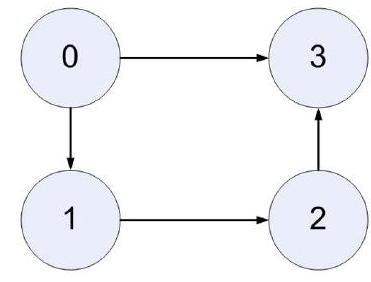
\includegraphics[max width=\textwidth]{2023_10_07_a50fd94fd281fe9896c1g-07(1)}
\end{center}

Fig. 2. Communication digraph between spacecraft.

\begin{center}
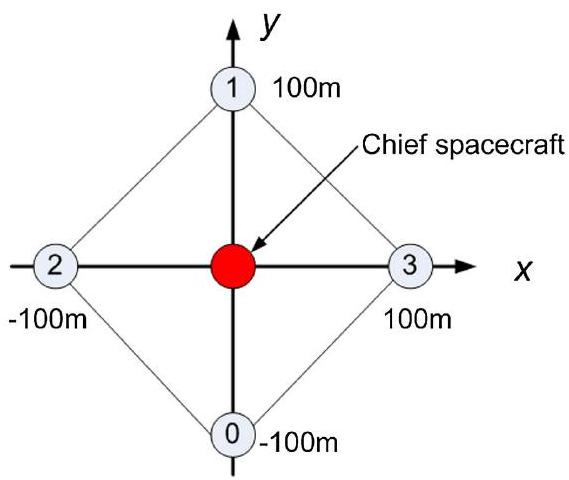
\includegraphics[max width=\textwidth]{2023_10_07_a50fd94fd281fe9896c1g-07(2)}
\end{center}

Fig. 3. Desired formation of the chief spacecraft and the spacecraft around it.

Since $\epsilon_{j}$ converges to zero, $\bar{q}_{j}$ converges to an identity quaternion, which means that $\tilde{q}_{j}$ converges to $\bar{\chi}_{j}$. So, $\tilde{q}_{j}$ converges to $\tilde{q}_{0}$. Therefore, Eq. (26) is satisfied.

Remark 4: The control laws for attitude control are distributed and Neighbors' information enters into the control law $\tau_{j}$ through $\xi_{j}$. In Theorem 2, it is assumed that the information of the leader is globally reachable to the followers (i.e., Assumption 4). If Assumption 4 is not satisfied, the attitudes of the followers cannot be synchronized with the attitude of the leader.

\section{Simulation}
Consider one chief spacecraft with four satellites around it. It is assumed that the chief spacecraft runs in an elliptical orbit with elements: $a_{r}=42241 \mathrm{~km}$, eccentricity $e_{l}=0.2$ and mean motion $n_{l}=7.2722 \times 10^{-5} \mathrm{rad}$. Based on Eqs. (2) and (3), we have

$$
\begin{gathered}
r_{r}=\frac{a_{r}\left(1-e_{l}^{2}\right)}{1+e_{l} \cos \nu(t)} \\
\dot{\nu}(t)=\frac{n_{l}\left(1+e_{l} \cos \nu\right)^{2}}{\left(1-e_{l}^{2}\right)^{3 / 2}} \\
\ddot{\nu}(t)=\frac{-2 n_{l}^{2} e_{l}\left(1+e_{l} \cos \nu\right)^{3} \sin \nu}{\left(1-e_{l}^{2}\right)^{3}}
\end{gathered}
$$

For the four spacecraft, there is one leader spacecraft (labeled by 0 ) and three follower spacecraft (labeled by 1, 2, and 3 ). For the follower spacecraft, it is assumed that $m_{j}=410 \mathrm{~kg}$, $F_{d j}=[-1.025,6.248,-2.415]^{\mathrm{T}} \times 10^{-5} \sin (j t) N$, the inertial moment $J_{j}=\operatorname{diag}([60,40,60]) \mathrm{kg} \cdot \mathrm{m}^{2}$, and the disturbance $\tau_{d j}=$ $[1.2 ;-2.1 ; 1.1] \times 10^{-5} \cos (j t) \mathrm{N} \cdot \mathrm{m}$ for $1 \leq j \leq 3$. The communications between the leader and follower spacecraft are shown in

\begin{center}
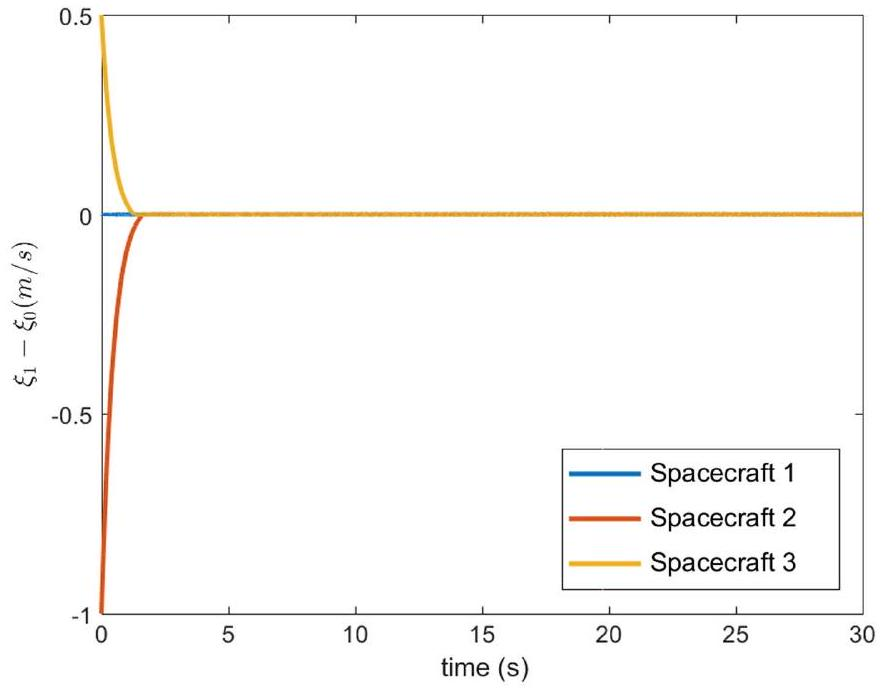
\includegraphics[max width=\textwidth]{2023_10_07_a50fd94fd281fe9896c1g-07(3)}
\end{center}

Fig. 4. Response of $\xi_{1}-\xi_{0}$.

\begin{center}
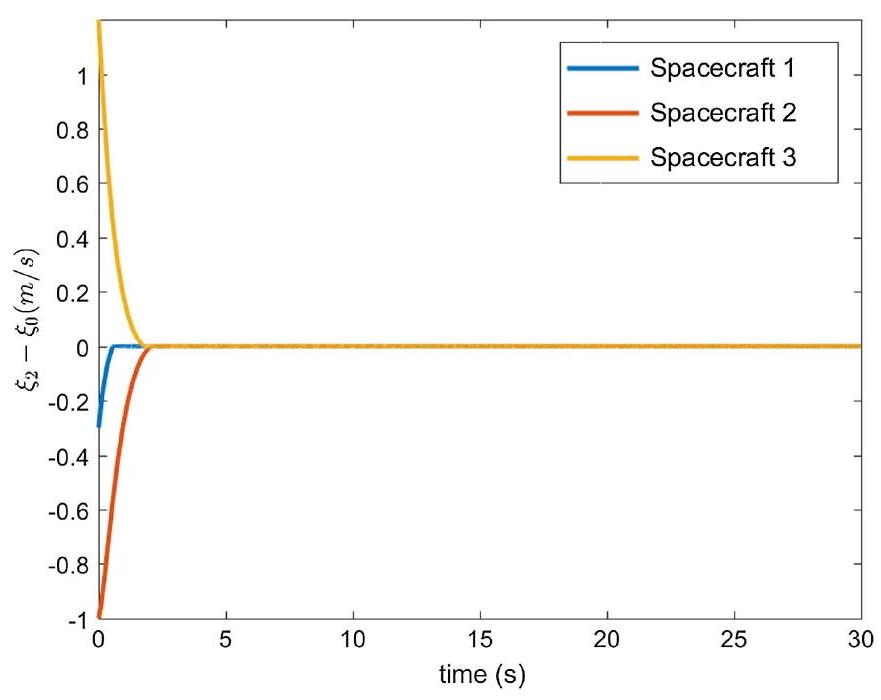
\includegraphics[max width=\textwidth]{2023_10_07_a50fd94fd281fe9896c1g-07}
\end{center}

Fig. 5. Response of $\xi_{2}-\xi_{0}$.

Fig. 2. The desired formation of the four spacecraft is shown in Fig. 3, where the chief spacecraft is located in the origin of the coordinate. In the simulation, the initial conditions of the follower spacecraft are: $\quad p_{1}(0)=[5,95,2]^{\mathrm{T}}, \quad \dot{p}_{1}(0)=[0.2,-0.2,0.1]^{\mathrm{T}}$, $\tilde{q}_{1}=[0.1,0.2,-0.2,0.95]^{\mathrm{T}}, \quad \tilde{\omega}_{1}=[-0.5,0.2,-0.1]^{\mathrm{T}} ; \quad p_{2}(0)=$ $[-96,5,-2]^{\mathrm{T}}, \quad \dot{p}_{2}(0)=[-0.2,0.2 ;, 0.2]^{\mathrm{T}}, \quad \tilde{q}_{2}=[0.1,-0.2,-$ $0.2,0.95]^{\mathrm{T}}, \tilde{\omega}_{2}=[0.5,-0.2,0.1]^{\mathrm{T}} ; p_{3}(0)=[97,-2,3]^{\mathrm{T}}, \dot{p}_{3}(0)=$ $[-0.3,0.4,-0.2]^{\mathrm{T}}, \quad \tilde{q}_{3}=[-0.1,-0.2,0.2,0.95]^{\mathrm{T}}$, and $\tilde{\omega}_{3}=[0.3$, $-0.3,0.2]^{\mathrm{T}}$, which means that the follower spacecraft are not in the desired formation and their attitudes are not synchronized. It is also assumed that the estimate mass of spacecraft $j$ is $\bar{m}_{j}=400 \mathrm{~kg}$ and the estimate inertia moment is $\bar{J}_{j}=$ $\operatorname{diag}([55,45,63]) \mathrm{kg} \cdot \mathrm{m}^{2}$ for $1 \leq j \leq 3$. The trajectory of the leader spacecraft is assumed to be $p_{0}(t)=(-100 \cos (0.01 t) m$, $100 \sin (0.01 t) m, 0 m)$ and the relative attitude is assumed to be $\tilde{q}(t)=[\cos (0.01 t), \sin (0.01 t), 0,0]^{\mathrm{T}}$.

With the aid of the results in Theorem 1, distributed robust controllers can be obtained for the formation flying. Figs. 4-6 show the

\begin{center}
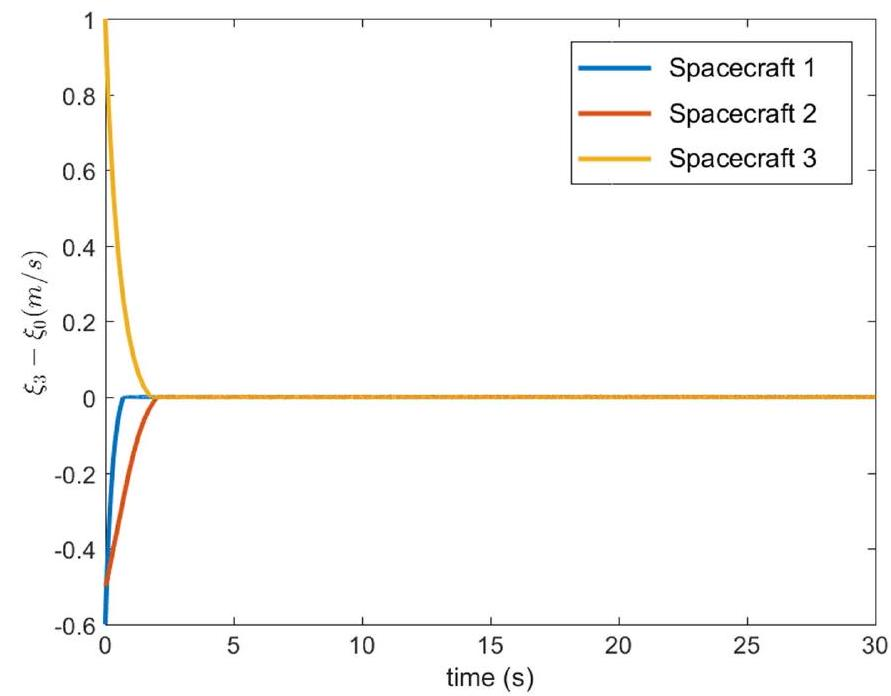
\includegraphics[max width=\textwidth]{2023_10_07_a50fd94fd281fe9896c1g-08(1)}
\end{center}

Fig. 6. Response of $\xi_{3}-\xi_{0}$.

\begin{center}
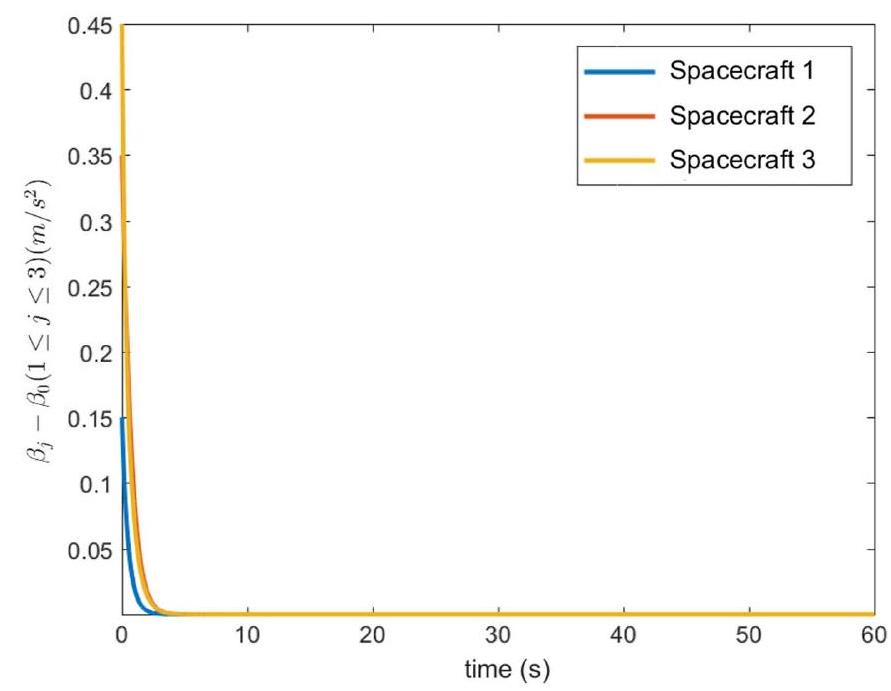
\includegraphics[max width=\textwidth]{2023_10_07_a50fd94fd281fe9896c1g-08(4)}
\end{center}

Fig. 7. Response of $\beta_{j}-\beta_{0}$ for $1 \leq j \leq 3$.

\begin{center}
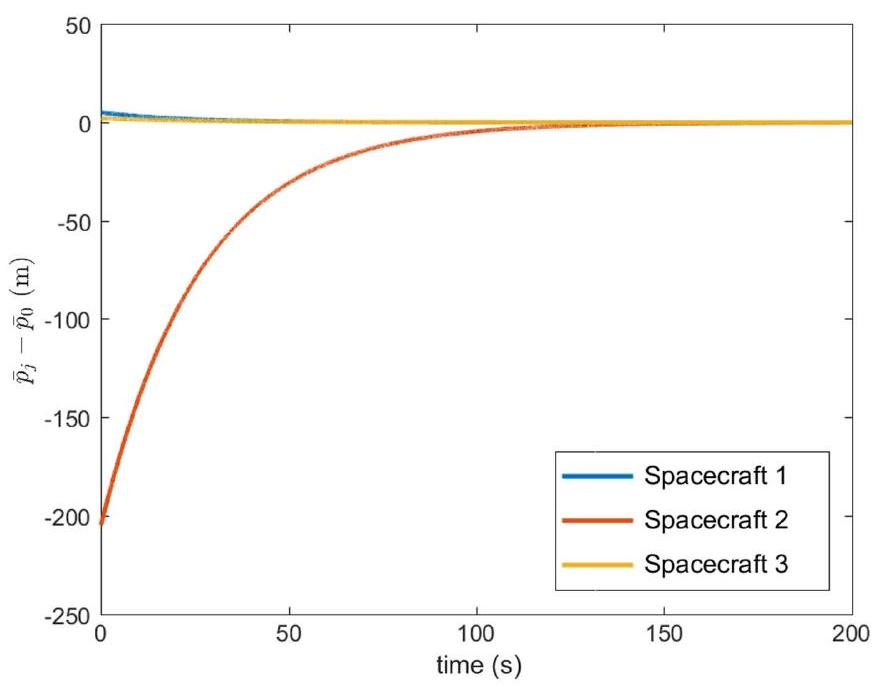
\includegraphics[max width=\textwidth]{2023_10_07_a50fd94fd281fe9896c1g-08}
\end{center}

Fig. 8. Tracking error of $\tilde{p}_{1}$.

\begin{center}
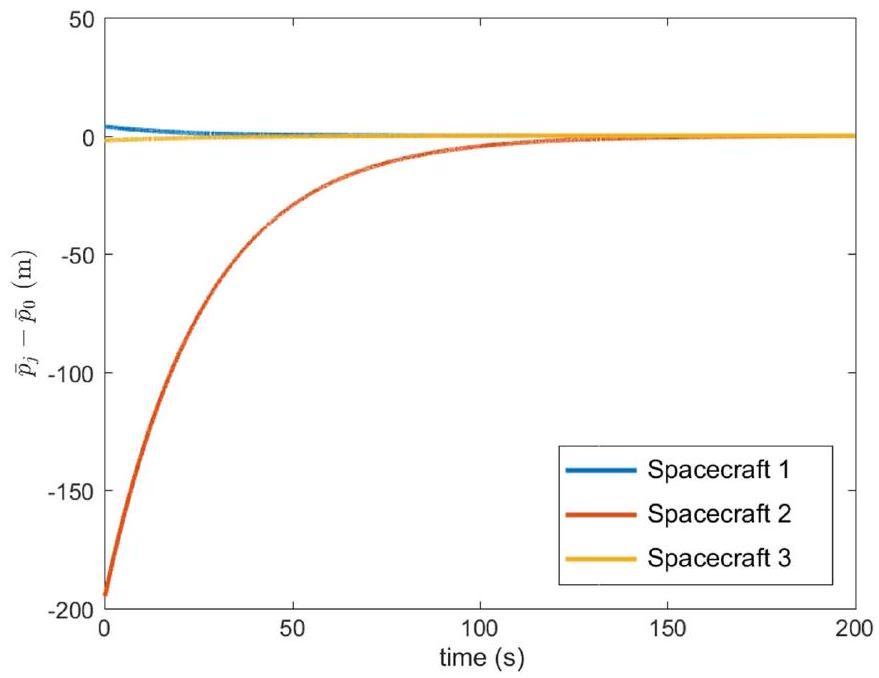
\includegraphics[max width=\textwidth]{2023_10_07_a50fd94fd281fe9896c1g-08(3)}
\end{center}

Fig. 9. Tracking error of $\tilde{p}_{2}$.

\begin{center}
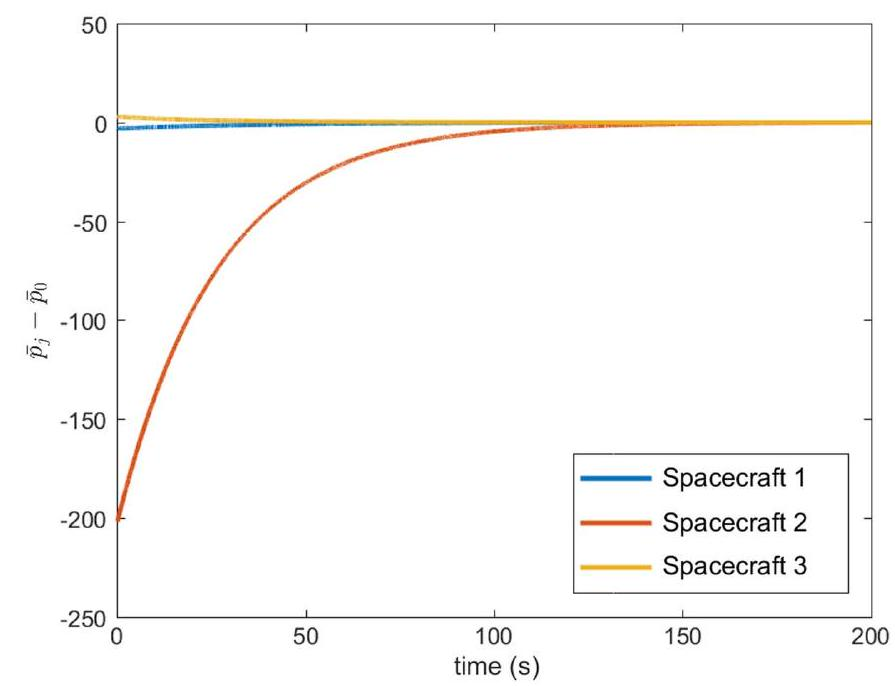
\includegraphics[max width=\textwidth]{2023_10_07_a50fd94fd281fe9896c1g-08(2)}
\end{center}

Fig. 10. Tracking error of $\tilde{p}_{3}$.

distributed estimate errors $\xi_{j}-\xi_{0}$ for $1 \leq j \leq 3$. It is shown that they converge to zero, which confirms the claims in Theorem 1. Fig. 7 shows the response of $\beta_{j}-\beta_{0}$ for $1 \leq j \leq 3$, which means the estimation errors converge to zero. Figs. 8-10 show the tracking errors $\tilde{p}_{j}$ for $1 \leq j \leq 3$. It is shown that all curves converge to zero. Therefore, the spacecraft come into the desired formation. In the simulation, the basis matrix $\phi_{j}$ was chosen as a $10 \times 3$ matrix with its elements being radial basis functions. The simulation results show that $\theta_{j}(1 \leq j \leq 3)$ are bounded, which are omitted due to too many figures.

For the attitude synchronization, distributed robust controllers can be obtained by Theorem 2. Figs. 11-13 show the distributed errors of $\chi_{j}-\chi_{0}$. It is shown that they all converge to zero. Fig. 14 shows the response of $\gamma_{j}-\gamma_{0}$ for $1 \leq j \leq 3$, which means the estimation errors converge to zero. Figs. $15-17$ show that response of $\tilde{q}_{j}$ for $1 \leq j \leq 3$. It shows that the first element of $\tilde{q}_{j}$ converges to one and the other elements converge to zero, which means that the attitude of each follower spacecraft converges to the attitude of the leader spacecraft. The simulation results show that the proposed control laws in Theorems 1 and 2 have the ability to ensure that

\begin{center}
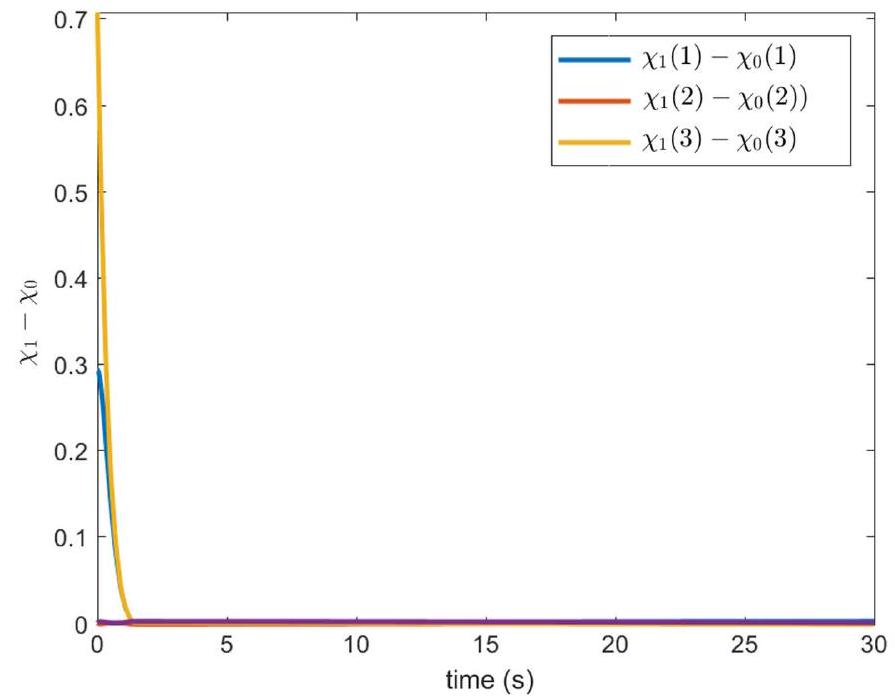
\includegraphics[max width=\textwidth]{2023_10_07_a50fd94fd281fe9896c1g-09(1)}
\end{center}

Fig. 11. Response of $\chi_{1}-\chi_{0}$.

\begin{center}
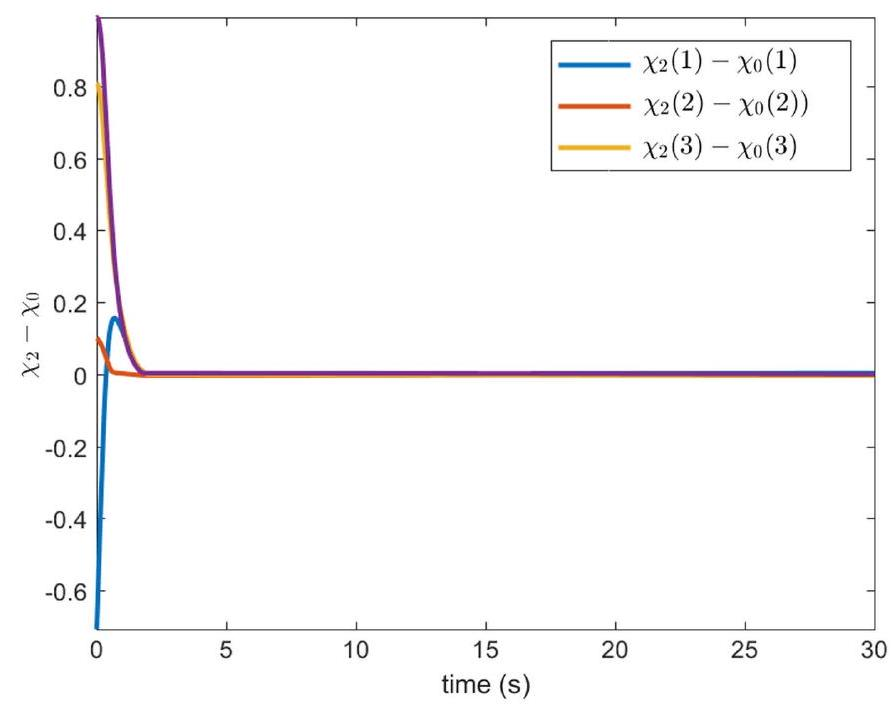
\includegraphics[max width=\textwidth]{2023_10_07_a50fd94fd281fe9896c1g-09(4)}
\end{center}

Fig. 12. Response of $\chi_{2}-\chi_{0}$.

\begin{center}
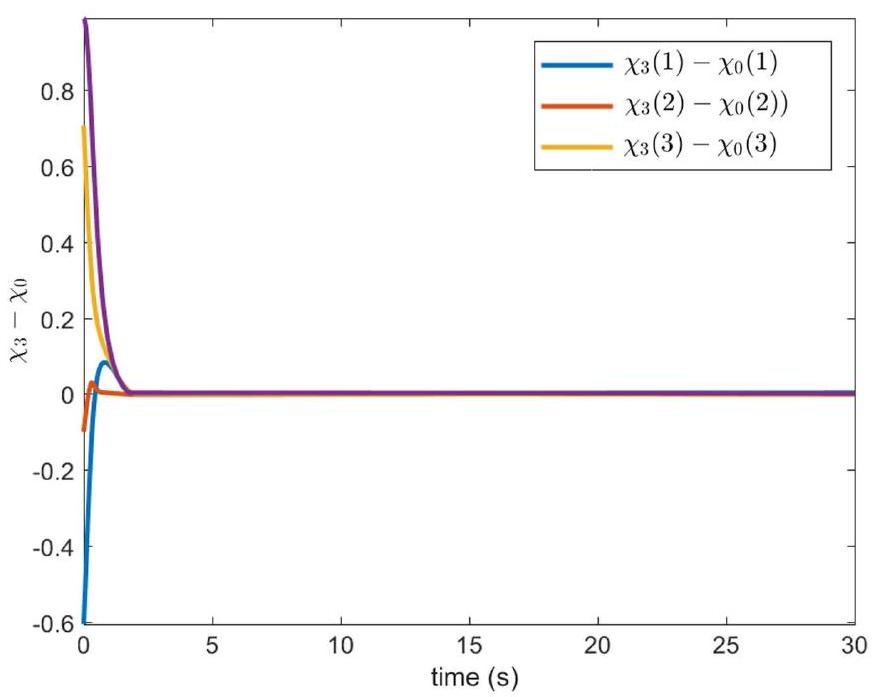
\includegraphics[max width=\textwidth]{2023_10_07_a50fd94fd281fe9896c1g-09(5)}
\end{center}

Fig. 13. Response of $\chi_{3}-\chi_{0}$.

\begin{center}
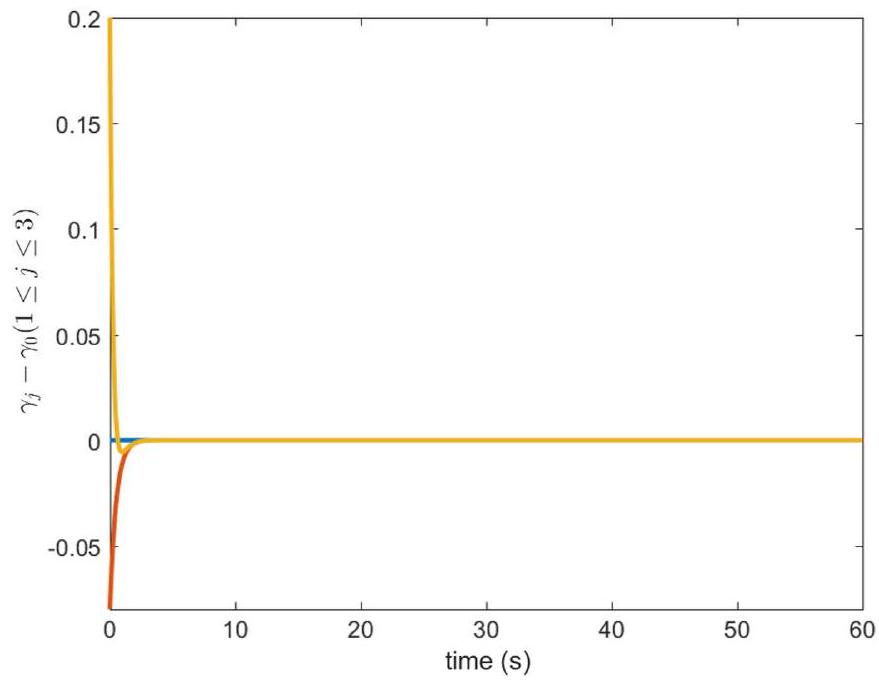
\includegraphics[max width=\textwidth]{2023_10_07_a50fd94fd281fe9896c1g-09(3)}
\end{center}

Fig. 14. Response of $\gamma_{j}-\gamma_{0}$ for $1 \leq j \leq 3$.

\begin{center}
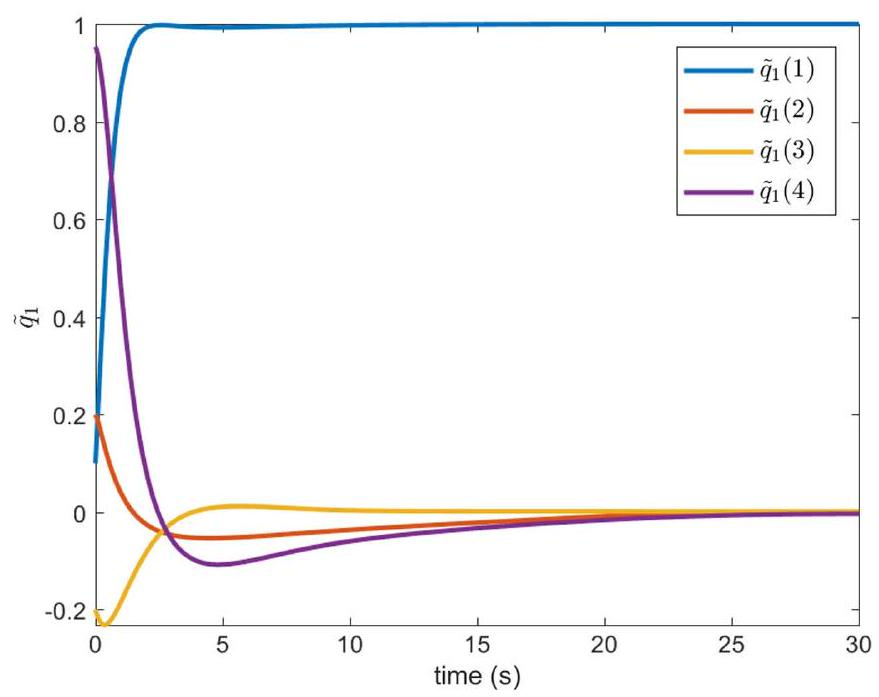
\includegraphics[max width=\textwidth]{2023_10_07_a50fd94fd281fe9896c1g-09(2)}
\end{center}

Fig. 15. Response of $\tilde{q}_{1}$.

\begin{center}
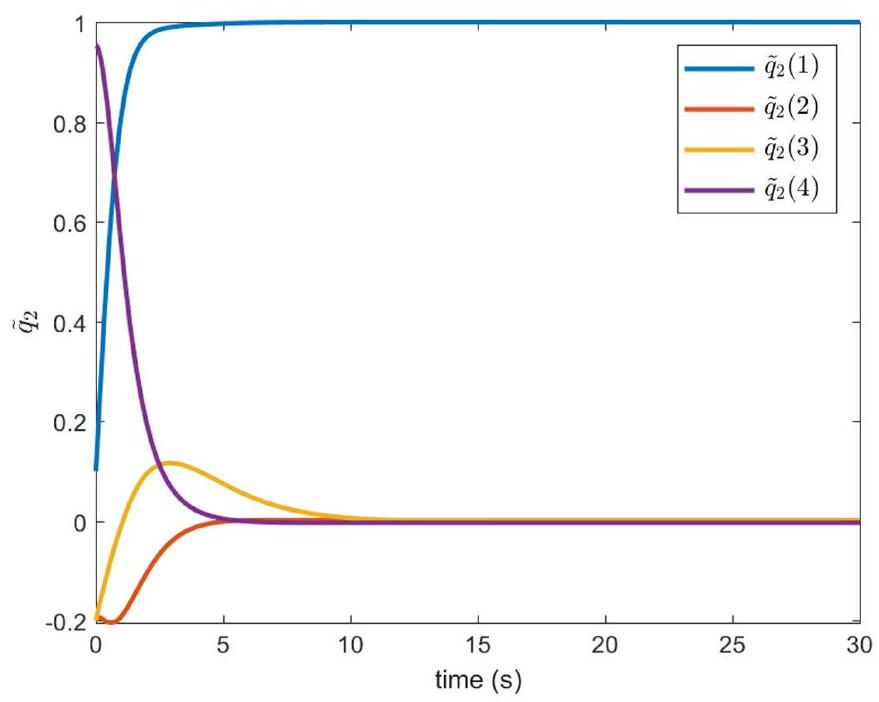
\includegraphics[max width=\textwidth]{2023_10_07_a50fd94fd281fe9896c1g-09}
\end{center}

Fig. 16. Response of $\tilde{q}_{2}$.

\begin{center}
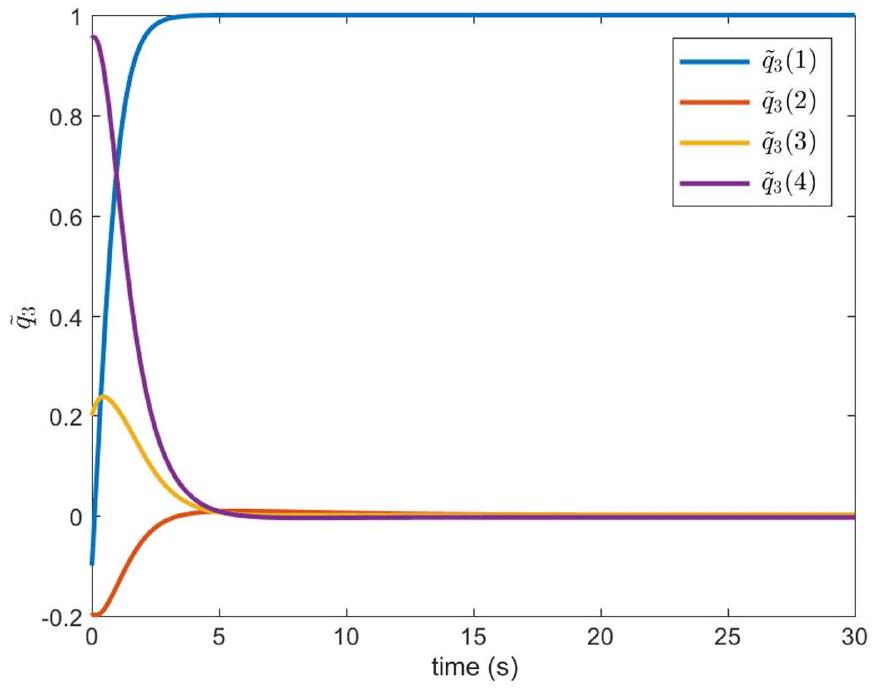
\includegraphics[max width=\textwidth]{2023_10_07_a50fd94fd281fe9896c1g-10}
\end{center}

Fig. 17. Response of $\tilde{q}_{3}$.

all spacecrafts move in a desired formation with the same attitude in the presence of uncertainties and orbital perturbations.

\section{Conclusion}
This paper studied the spacecraft formation flying with a desired attitude. Distributed control laws were proposed for relative translation of multiple spacecraft such that the spacecraft come into a desired formation when there is parametric uncertainty and nonparametric uncertainty. For the attitude synchronization of multiple spacecraft distributed control laws were also proposed such that the attitudes of the follower spacecraft converge to the attitude of the leader spacecraft when there is uncertainty in the dynamics. The simulation results show the effectiveness of the proposed control algorithms.

\section{Data Availability Statement}
Some or all data, models, or code that support the findings of this study are available from the corresponding author upon reasonable request.

\section{References}
Balch, T., and R. C. Arkin. 1998. "Behavior-based formation control for multirobot teams." IEEE Trans. Rob. Autom. 14 (6): 926-939. https:// \href{http://doi.org/10.1109/70.736776}{doi.org/10.1109/70.736776}.

Beard, R. W., J. Lawton, and F. Y. Hadaegh. 2001. "A coordination architecture for spacecraft formation control." IEEE Trans. Control Syst. Technol. 9 (6): 777-790. \href{https://doi.org/10.1109/87.960341}{https://doi.org/10.1109/87.960341}.

Cao, Y., and W. Ren. 2010a. "Distributed coordinated tracking via a variable structure approach. Part I: Consensus tracking." In Proc., American Control Conf., 4744-4749. Arlington, VA: American Automatic Control Council.

Cao, Y., and W. Ren. 2010b. "Distributed coordinated tracking via a variable structure approach. Part II: Swarm tracking." In Proc., American Control Conf., 4750-4755. Arlington, VA: American Automatic Control Council.

Clohessy, W. H., and R. S. Wiltshire. 1960. "Terminal guidance system for satellite rendezvous.” J. Aerosp. Sci. 27 (9): 653-658. \href{https://doi.org/10}{https://doi.org/10} $.2514 / 8.8704$
Das, A. K., R. Fierro, and V. Kumar. 2002. Cooperative control and optimization of applied optimization, in control graphs for robot networks. Norwell, MA: Kluwer.

Desai, J., J. Ostrowski, and V. Kumar. 1998. "Controlling formations of multiple mobile robots." In Proc., IEEE Int. Conf. on Robotics and Automation, 2864-2869. New York: IEEE.

Desai, J. P., J. P. Ostrowski, and V. Kumar. 2001. "Modeling and control of formations of nonholonomic mobile robots." IEEE Trans. Rob. Autom. 17 (6): 905-908. \href{https://doi.org/10.1109/70.976023}{https://doi.org/10.1109/70.976023}.

Dong, W. 2013. "Distributed tracking control of networked chained systems." Int. J. Control 86 (12): 2159-2174. \href{https://doi.org/10.1080}{https://doi.org/10.1080} /00207179.2013.803156.

Eren, T., P. N. Belhumeur, and A. S. Morse. 2002. "Closing ranks in vehicle formations based on rigidity." In Proc., IEEE Conf. on Decision and Control, 2959-2964. New York: IEEE.

Fax, J. A., and R. M. Murray. 2004. "Information flow and cooperative control of vehicle formations." IEEE Trans. Autom. Contr. 49 (9): 1465-1476. \href{https://doi.org/10.1109/TAC.2004.834433}{https://doi.org/10.1109/TAC.2004.834433}.

Haizhou, P., and V. Kapila. 2001. "Adaptive nonlinear control for spacecraft formation flying with coupled translational and attitude dynamics." In Vol. 3 of Proc., 40th IEEE Conf. on Decision and Control, 2057-2062. New York: IEEE.

Hong, Y., G. R. Chen, and L. Bushnell. 2008. "Distributed observers design for leader-following control of multi-agent." Automatica 44 (3): 846-850. \href{https://doi.org/10.1016/j.automatica.2007.07.004}{https://doi.org/10.1016/j.automatica.2007.07.004}.

Hong, Y., J. Hu, and L. Gao. 2006. "Tracking control for multi-agent consensus with an active leader and variable topology." Automatica 42 (7): 1177-1182. \href{https://doi.org/10.1016/j.automatica.2006.02.013}{https://doi.org/10.1016/j.automatica.2006.02.013}.

Jonathan, R. T., J. Lawton, R. W. Beard, and B. J. Young. 2003. "A decentralized approach to formation maneuvers." IEEE Trans. Rob. Autom. 19 (6): 933-941. \href{https://doi.org/10.1109/TRA.2003.819598}{https://doi.org/10.1109/TRA.2003.819598}.

Kapilal, V., A. G. Sparks, J. M. Buffington, and Q. Yan. 1999. "Spacecraft formation flying: Dynamics and control.” In Vol. 6 of Proc., 1999 American Control Conf., 4137-4141. Arlington, VA: American Automatic Control Council.

Kristiansen, R., P. J. Nicklasson, and J. T. Gravdahl. 2008. "Spacecraft coordination control in 6DOF: Integrator backstepping vs passivity-based control." Automatica 44 (11): 2896-2901. \href{https://doi.org/10.1016/j}{https://doi.org/10.1016/j} .automatica.2008.04.019.

Lafferriere, G., J. Caughman, and A. Williams. 2004. "Graph theoretic methods in the stability of veicle formations." In Proc., American Control Conf., 3729-3734. Arlington, VA: American Automatic Control Council.

Lafferriere, G., A. Williams, J. Caughman, and J. J. P. Veermany. 2005. "Decentralized control of vehicle formations." Syst. Control Lett. 54 (9): 899-910. \href{https://doi.org/10.1016/j.sysconle.2005.02.004}{https://doi.org/10.1016/j.sysconle.2005.02.004}.

Lan, Q., J. Yang, S. Li, and H. Sun. 2015. "Finite-time control for 6 DOF spacecraft formation flying systems." J. Aerosp. Eng. 28 (5): 04014137. \href{https://doi.org/10.1061/(ASCE)AS.1943-5525.0000476}{https://doi.org/10.1061/(ASCE)AS.1943-5525.0000476}.

Lawton, J., R. W. Beard, and B. Young. 2003. "A decentralized approach to formation maneuvers." IEEE Trans. Rob. Autom. 19 (6): 933-941. \href{https://doi.org/10.1109/TRA.2003.819598}{https://doi.org/10.1109/TRA.2003.819598}.

Lee, T., and H. Ahn. 2010. "Consensus of nonlinear system using feedback linearization.” In Proc., 2010 IEEE/ASME Int. Conf. on Mechatronic and Embedded Systems and Applications. New York: IEEE.

Lewis, M. A., and K.-H. Tan. 1997. "High precision formation control of mobile robots using virtual structures." Auton. Robots 4 (4): 387-403. \href{https://doi.org/10.1023/A:1008814708459}{https://doi.org/10.1023/A:1008814708459}.

Li, Z., Z. Duan, G. Chen, and L. Huang. 2010. "Consensus of multiagent systems and synchronization of complex networks: A unified viewpoint.” IEEE Trans. Circuits Syst. I Regul. Pap. 57 (1): 213-224. \href{https://doi.org/10.1109/TCSI.2009.2023937}{https://doi.org/10.1109/TCSI.2009.2023937}.

Lv, Y., Q. Hu, G. Ma, and J. Zhou. 2011. "6 DOF synchronized control for spacecraft formation flying with input constraint and parameter uncertainties." ISA Trans. 50 (4): 573-580. \href{https://doi.org/10.1016/j.isatra}{https://doi.org/10.1016/j.isatra} .2011.04.001.

Mei, J., W. Ren, and G. Ma. 2011. "Distributed coordinated tracking with a dynamic leader for multiple euler-lagrange systems." IEEE Trans. Autom. Control 56 (6): 1415-1421. \href{https://doi.org/10.1109/TAC.2011}{https://doi.org/10.1109/TAC.2011} .2109437 . Mercier, M., S. Phillips, M. Shubert, and W. Dong. 2020. "Terrestrial testing of multi-agent, relative guidance, navigation, and control algorithms." In Proc., 2020 IEEE/ION Position, Location and Navigation Symp., 1488-1497. New York: IEEE.

Mesbahi, M., and F. Y. Hadaegh. 2001. "Formation flying control of multiple spacecraft via graphs, matrix inequalities, and switching." AIAA $J$. Guidance Control Dyn. 24 (2): 369-377. \href{https://doi.org/10.2514/2}{https://doi.org/10.2514/2} .4721 .

Olfati-Saber, R., and R. M. Murray. 2002. "Distributed structural stabilization and tracking for formations of dynamic multiagents." In Proc., IEEE Conf. Decision and Control, 209-215. New York: IEEE.

$\mathrm{Qu}, \mathrm{Z}$. 2009. Cooperative control of dynamical systems: Applications to autonomous vehicles. New York: Springer.

Qu, Z. 2010. "Cooperative control of networked nonlinear systems." In Proc., 49th IEEE Conf. on Decision and Control. New York: IEEE.

Ren, W., and R. W. Beard. 2004. "Formation feedback control for multiple spacecraft via virtual structures." IEE Proc., Control Theory Appl. 151 (3): 357-368. \href{https://doi.org/10.1049/ip-cta:20040484}{https://doi.org/10.1049/ip-cta:20040484}.

Ren, W., and R. W. Beard. 2005. "Consensus seeking in multi-agent systems under dynamically changing interaction topologies." IEEE Trans. Autom. Control 50 (5): 655-661. \href{https://doi.org/10.1109/TAC.2005}{https://doi.org/10.1109/TAC.2005} .846556 .

Scardovi, L., and R. Sepulchre. 2009. "Synchronization in networks of identical linear systems." Automatica 45 (11): 2557-2562. \href{https://doi}{https://doi} .org/10.1016/j.automatica.2009.07.006.

Sugihara, K., and I. Suzuki. 1996. "Distributed algorithms for formation of geometric patterns with many mobile robots." J. Rob. Syst. 13 (3):
127-139. \href{https://doi.org/10.1002/(SICI)1097-4563(199603)13:3}{https://doi.org/10.1002/(SICI)1097-4563(199603)13:3}<127: AID-ROB1>\href{http://3.0.CO}{3.0.CO};2-U.

Sun, H., S. Li, and S. Fei. 2011. "A composite control scheme for 6DOF spacecraft formation control." Acta Astronaut. 69 (7): 595-611. https:// \href{http://doi.org/10.1016/j.actaastro.2011.04.009}{doi.org/10.1016/j.actaastro.2011.04.009}.

Wang, J., and Z. Sun. 2012. "6-DOF robust adaptive terminal sliding mode control for spacecraft formation flying." Acta Astronaut. 73 (Apr-May): 76-87. \href{https://doi.org/10.1016/j.actaastro.2011.12.005}{https://doi.org/10.1016/j.actaastro.2011.12.005}.

Wang, P. K. C., and F. Y. Hadaegh. 1996. "Coordination and control of multiple microspacecraft moving in formation." J. Astronaut. Sci. 44 (3): 315-355.

Wieland, P., R. Sepulchre, and F. Allgower. 2011. "An internal model principle is necessary and sufficient for linear output synchronization." Automatica 47 (5): 1068-1074. \href{https://doi.org/10.1016/j.automatica}{https://doi.org/10.1016/j.automatica} 2011.01.081.

Yan, Q., G. Yang, V. Kapila, and M. S. de Queiroz. 2000a. "Nonlinear dynamics and output feedback control of multiple spacecraft in elliptical orbits." In Vol. 2 of Proc., 2000 American Control Conf., 839-843. Arlington, VA: American Automatic Control Council.

Yan, Q., G. Yang, V. Kapila, and M. Queiroz. 2000b. "Nonlinear dynamics, trajectory generation, and adaptive control of multiple spacecraft in periodic relative orbits." In Proc., AAS Guidance and Control Conf., 159-173. San Diego: American Astronautical Society.

Zhang, H., and F. L. Lewis. 2012. "Adaptive cooperative tracking control of higher-order nonlinear systems with unknown dynamics." Automatica 48 (7): 1432-1439. \href{https://doi.org/10.1016/j.automatica.2012.05.008}{https://doi.org/10.1016/j.automatica.2012.05.008}.


\end{document}